\documentclass[11pt]{article}
\usepackage{amsmath}
\usepackage{amsfonts}
\usepackage{bm}
\usepackage{url}
\usepackage{fancyvrb}
\usepackage{graphicx}
\usepackage{float}
\begin{document}

\title{Stochastic Networks HW 3}
\author{Zane Jakobs}
\date{}
\maketitle
NOTE: for some reason, the code didn't format correctly in this document, so if you want to read it, I recommend just reading the files from either my email or my GitHub.
\subsection*{1} I am planning to do the project we originally discussed, a traffic model. Specifically, I will be using PETSc's DMNetwork class to write a distributed traffic model to simulate traffic wait times, vehicle miles traveled, and other similar quantities. The US Federal Highway Administration makes traffic monitoring data available at \url{https://www.fhwa.dot.gov/policyinformation/tables/tmasdata/}, which can be assimilated with a variety of methods (e.g. 4DVAR, various ensemble Kalman methods) to estimate the state of the traffic system under various different assumptions; for example, one might know that the arrival distribution of cars in a certain region is, say, Poisson distributed with a well-estimated mean $\Lambda$. The model will in theory be able to be configured to run both short-term traffic forecasts and longer-term analyses, but this is largely a function of the data assimilation techniques used instead of the network modeling techniques (which is in turn largely a function of available compute and model size).

\subsection*{2(a)} The following C function places the value of $h(p)$ into the variable $k$ (of type PetscInt*):\\
\begin{Verbatim}[xleftmargin=-1cm]
static PetscErrorCode ChungLuInvCDF(PetscReal p, PetscInt* k, PetscInt k0,
				PetscInt n, PetscReal gamma)
{
/* solves ChungLuCDF(k) = p */
PetscReal cfactor, kc;

cfactor = 1.0/(pow((PetscReal)k0, 1.0-gamma) - pow((PetscReal)n, 1.0-gamma));

if(gamma > 1.0){
kc = pow(p/cfactor, 1.0/(1.0 - gamma ));
} else {

kc = pow(p, 1.0/(1.0 - gamma)) / pow(cfactor, 1.0/(1.0 - gamma));
}

if(kc > n){
kc = n;
} 
else if( kc < k0 ){
kc = k0;
}

*k = round(kc);

return(0);
}
\end{Verbatim}
\subsection*{2(b)} Such a network can be generated by running the HW3 executable (makefile and code are at the end of the assignment and on my Github, \url{https://github.com/diffeoinvariant/Stochastic-Networks}) with the arguments 
\begin{Verbatim}
./HW3 -n 2000 -k0 20 -g 4.0
\end{Verbatim}
and gives the following answers (for the network it generated on this run; as it's stochastic, results may vary slightly)
\begin{Verbatim}
<kin, kout> = 209.711000 
<k> = 14.566000 
, <kin,kout>/<k> = 14.397295 .
Largest eigenvalue: 14.955780
\end{Verbatim}

\subsection*{2(c)} We get the following plots:
\begin{figure}[H]
\includegraphics[scale=0.7]{HW/g4targ}
\label{fig:g4targ}	
\end{figure}
\begin{figure}[H]
	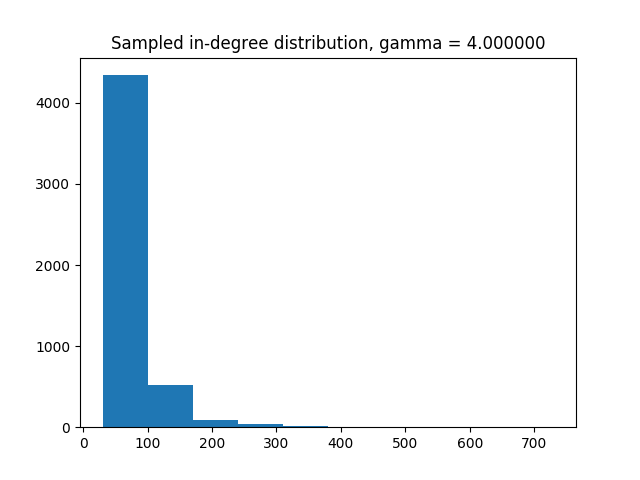
\includegraphics[scale=0.7]{HW/g4sample}
	\label{fig:g4sample}	
\end{figure}
\begin{figure}[H]
	\includegraphics[scale=0.7]{HW/g4scatter}
	\label{fig:g4scatter}	
\end{figure}
\begin{figure}[H]
	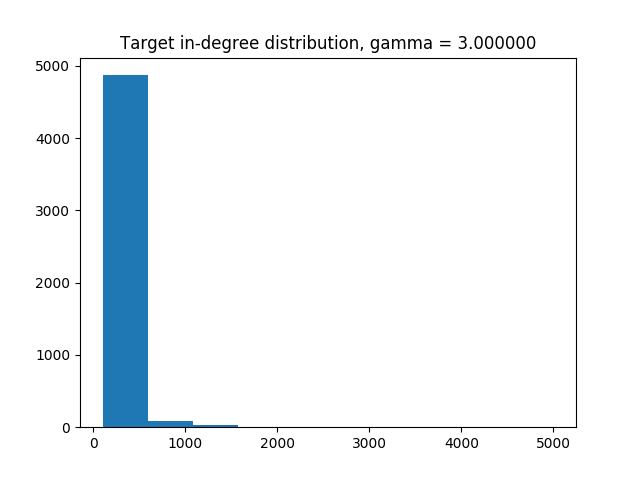
\includegraphics[scale=0.7]{HW/g3targ}
	\label{fig:g3targ}	
\end{figure}
\begin{figure}[H]
	\includegraphics[scale=0.7]{HW/g3sample}
	\label{fig:g3sample}	
\end{figure}
\begin{figure}[H]
	\includegraphics[scale=0.7]{HW/g3scatter}
	\label{fig:g3scatter}	
\end{figure}
\begin{figure}[H]
	\includegraphics[scale=0.7]{HW/g25targ}
	\label{fig:g25targ}	
\end{figure}
\begin{figure}[H]
	\includegraphics[scale=0.7]{HW/g25sample}
	\label{fig:g25sample}	
\end{figure}
\begin{figure}[H]
	\includegraphics[scale=0.7]{HW/g25scatter}
	\label{fig:g25scatter}	
\end{figure}
\begin{figure}[H]
	\includegraphics[scale=0.7]{HW/g2targ}
	\label{fig:g2targ}	
\end{figure}
\begin{figure}[H]
	\includegraphics[scale=0.7]{HW/g2sample}
	\label{fig:g2sample}	
\end{figure}
\begin{figure}[H]
	\includegraphics[scale=0.7]{HW/g2scatter}
	\label{fig:g2scatter}	
\end{figure}

In general, the sampled degree distributions match the target very well in aggregate (in a histogram), but the individual nodes' target and sampled degrees don't appear to be particularly well-correlated in any of the plots.
\subsection*{3(a)} $k^{in}_{n,i} = \sum\limits_{i=1}^n a_ib_j,$ and $k^{in}_{n,i} = \sum\limits_{i=1}^n a_jb_i.$
\subsection*{3(b)} $\langle k\rangle = \dfrac{1}{N}\sum\limits_{i=1}^N \sum\limits_{j=1}^N a_i b_j$
\subsection*{3(c)} $\dfrac{\langle k^{in}_n k^{out}_n\rangle}{\langle k \rangle}  =  N\dfrac{\sum\limits_{i=1}^n\sum\limits_{j=1}^n a_ia_jb_ib_j}{\sum\limits_{i=1}^N\sum\limits_{j=1}^N a_i b_j}$
\subsection*{3(d)} First, choose $N-1$ linearly independent vectors that are orthogonal to $\bm{b}$; they clearly have eigenvalue 0. Now, the remaining nonzero eigenvalue can be found by considering the action of the matrix,
\[
(\bm{a}\bm{b}^T)\bm{u} = (\bm{b}^T\bm{u})\bm{a},
\]
and the eigenvalue equation
\[
(\bm{a}\bm{b}^T)\bm{u} = \lambda \bm{u},
\]
from which we can see that the eigenvalue we seek is $\lambda = \bm{a}^T\bm{b},$ the corresponding right eigenvector is $\bm{u} = \bm{a}$, and the left eigenvector is $\bm{v}^T = \bm{b}^T$.
\subsection*{4(a)} The Jacobian is $J = K\bm{A} - (1+2\bm{x})\bm{I}$, so its eigenvalues are the sums of the eigenvalues of $K\bm{A}$ and of $-(1+2\bm{0})\bm{I}$, which are all $-1$, so the Jacobian has all negative (real parts of its) eigenvalues (and thus the fixed point is stable) iff the largest eigenvalue of $K\bm{A}$, $\lambda_{\text{max}} \approx  \frac{\langle\hat{k_{in}}\hat{k_{out}}\rangle}{\langle k \rangle}$, is less than 1.
\subsection*{4(b)} We get the following plot for the norm of $x$ at $t=10$ versus $K$:\\
\begin{figure}[H]
	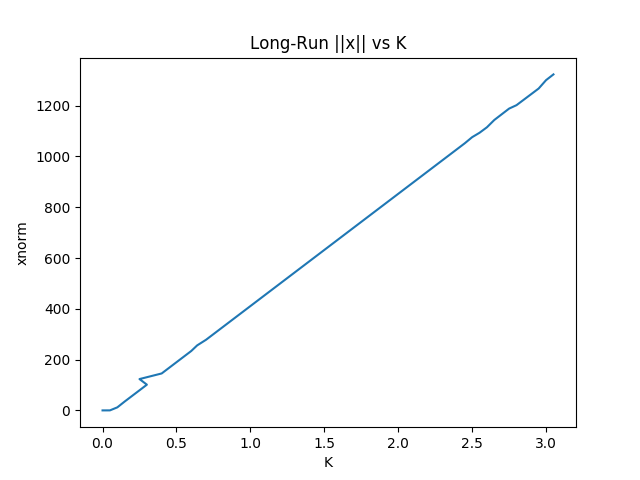
\includegraphics[scale=0.7]{HW/hw3p4res}
	\label{fig:hw3p4res}
\end{figure}
and at more fine resolution in the region of interest:\\
\begin{figure}[H]
	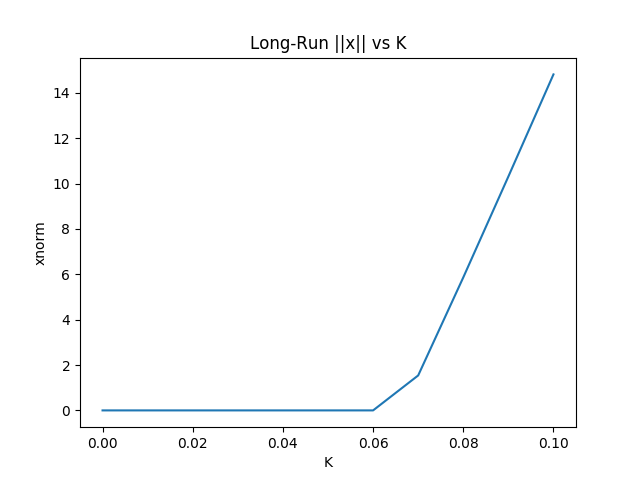
\includegraphics[scale=0.7]{HW/hw3p4resfine}
	\label{fig:hw3p4resfine}
\end{figure}

\subsection*{4(d)} Given that the largest eigenvalue (with the $\dfrac{\langle k_{in}k_{out}\rangle}{\langle k \rangle}$ approximation) is about $14.4$ (see problem 2(b); this is the same network), we should have $K_c\approx \frac{1}{14.4} \approx 0.0694.$ This agrees well with the plots we generated above.
\subsection*{5(a)} Plotting the real parts of the eigenvalues on the x axis and the imaginary parts on the y axis gives the following plot for $A$:
\begin{figure}[H]
	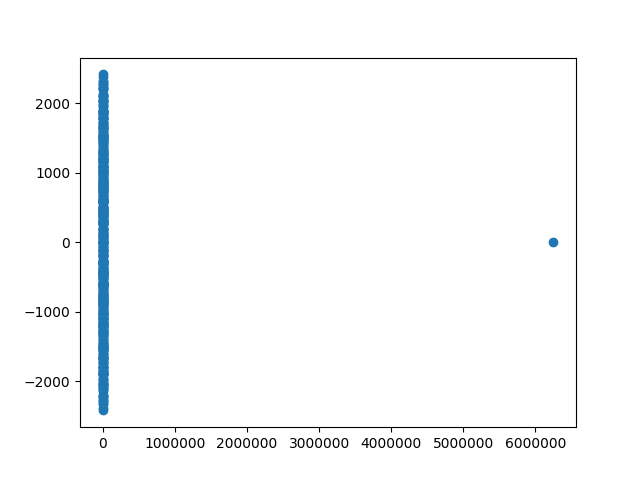
\includegraphics[scale=0.7]{HW/hw3p5realmat}
	\label{fig:hw3p5realmat}
\end{figure}
Indeed, we do get that one large, real eigenvalue!

\subsection*{5(b)}
We get the same for a variety of small epsilon, with plots looking like this:\\
\begin{figure}[H]
	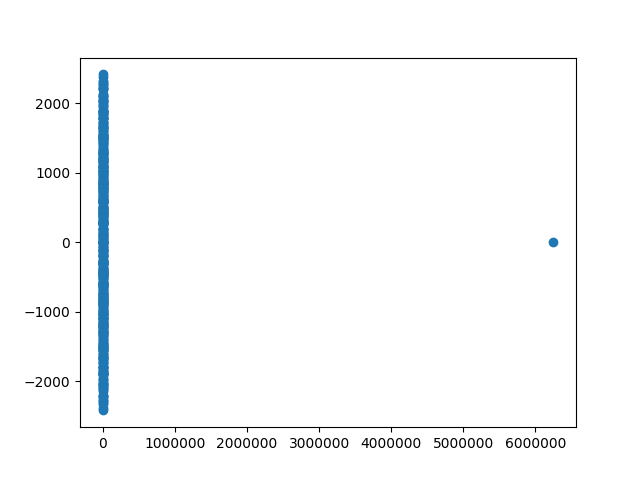
\includegraphics[scale=0.7]{HW/hw3p5}
	\label{fig:hw3p5}
\end{figure}


\section*{Code}
\subsection*{PETSc Code (Network generation, ODE solve)}
\begin{Verbatim}[xleftmargin=-3cm]
static char help[] = "Homework 3 Problem 4 code. Solves x' = kAx - x^2 - x for scalar k and graph adjacency matrix A.\n\
Input parameters:\n\
-k : scalar parameter\n\
-monitor (bool) : monitor the solver's progress and print to console? Default false.\n\
-n (int) : number of nodes in the network.\n\
--filename (same as -f) : filename for the adjacency matrix.\n\n";

#include <petscts.h> //PETSc time steppers
#include <petscsys.h>
#include <petscmat.h>
#include <mpi.h>
#include <math.h>
#include <stdbool.h>
#include <stdlib.h>
#include <limits.h>
#include <float.h>
#include <time.h>
/**
*
* We're solving the system of ODEs 
*
* x' = k * Ax - x - x^2
*
* for scalar k and adjacency matrix A.
*/

/*problem context struct*/  
typedef struct _n_prob_info *User;

struct _n_prob_info
{
Mat A; /* adjacency matrix */
PetscReal k, gamma; /* k factor in the above ODE */
PetscInt  k0, n;
/*bool print = true; print problem progress/info as it's being solved?*/

/*	long int max_timesteps = 1E6;*/
long int num_timesteps;
PetscReal next_output; /*for adjoint stuff*/
PetscReal tprev;
/*	long int  N;problem size*/
};

/*function that computes F(x,t) for system X' = F(X,t) */
static PetscErrorCode RHSFunction(TS ts, PetscReal t, Vec X, Vec F, void* ctx)
{
PetscErrorCode     ierr;
User               prob = (User)ctx;
PetscScalar    	   *f;
const PetscScalar  *x;
PetscScalar 	   xval;
PetscInt	   N, id;

ierr = MatMult(prob->A, X, F);CHKERRQ(ierr);
ierr = VecScale(F, prob->k);CHKERRQ(ierr);

VecGetArrayRead(X, &x);
VecGetArray(F, &f);
VecGetSize(F, &N);

for(id = 0; id < N; ++id){
xval = x[id];
f[id] -= xval + xval * xval;
}

VecRestoreArrayRead(X, &x);
VecRestoreArray(F, &f);

return(0);
}

/* Jacobian of RHS, dF/dX = k * A - (1-2x) * I */
static PetscErrorCode RHSJacobian(TS ts, PetscReal t, Vec X, Mat J, Mat Z, void* ctx)
{
PetscErrorCode     ierr;
User               prob = (User)ctx;
Mat 		   AminusJ;
Vec                IdMultVec;
PetscInt           N;

VecGetSize(X, &N);
/* get vector of 1 - 2x */
VecDuplicate(X, &IdMultVec);
VecSet(IdMultVec, 1.0);
ierr = VecAXPY(IdMultVec, -2.0, X);CHKERRQ(ierr);

/* insert IdMultVec into the diagonal of AminusJ = (1-2x)* I */
ierr = MatCreateAIJ(PETSC_COMM_WORLD, PETSC_DECIDE, PETSC_DECIDE, N, N, 1, NULL, 0, NULL, &AminusJ);CHKERRQ(ierr);
ierr = MatDiagonalSet(AminusJ, IdMultVec, INSERT_VALUES);CHKERRQ(ierr);
/* compute Jacobian */
MatDuplicate(prob->A, MAT_COPY_VALUES, &J);
ierr = MatScale(J, prob->k);CHKERRQ(ierr);
ierr = MatAXPY(J, -1.0, AminusJ, DIFFERENT_NONZERO_PATTERN);CHKERRQ(ierr);

if(Z != J){
MatAssemblyBegin(Z, MAT_FINAL_ASSEMBLY);
MatAssemblyEnd(Z, MAT_FINAL_ASSEMBLY);
}
MatDestroy(&AminusJ);
VecDestroy(&IdMultVec);
return(0);
}

/* Jacobian of RHS w.r.t. the parameter k, J_k = k * Ax */
static PetscErrorCode RHSJacobianP(TS ts, PetscReal t, Vec X, Mat J, void* ctx)
{
PetscErrorCode     ierr;
User               prob = (User)ctx;
PetscInt           id, idStart, idEnd, idLen, cols[]={0};
Vec                ax;


ierr = MatMult(prob->A, X, ax);CHKERRQ(ierr);

VecGetOwnershipRange(X, &idStart, &idEnd);
idLen = idEnd - idStart;
PetscInt rows[idLen];
for(id = 0; id < idLen; ++id){
rows[id] = id + idStart;
}

const PetscScalar  *Jvals;


VecGetArrayRead(ax, &Jvals);
MatSetValues(J, idLen,rows, 1, cols, Jvals, INSERT_VALUES);	

MatAssemblyBegin(J, MAT_FINAL_ASSEMBLY);
MatAssemblyEnd(J, MAT_FINAL_ASSEMBLY);


VecRestoreArrayRead(ax, &Jvals);
VecDestroy(&ax);

return(0);
}


static PetscErrorCode Monitor(TS ts, PetscInt step, PetscReal t, Vec X, void* ctx)
{
PetscErrorCode 		ierr;
PetscReal 		dt, tprev;      
User      		prob = (User)ctx; 

TSGetTimeStep(ts, &dt);
TSGetPrevTime(ts, &tprev);
/*
tsteps = prob->num_timesteps;

if(tsteps == 0){
// initial condition has not been set, error! 
return(-1); //I should figure out what the appropriate PETSc error code here is, but this should never happen anyway...
}
else if(tsteps >= prob->max_timesteps - 1){
//same
return(-1);
}
prob->tprev = tprev;
prob->t[tsteps] = tprev + dt;

prob->xs[tsteps] = X;
prob->num_timesteps++;
*/
PetscPrintf(PETSC_COMM_WORLD, "[%.1f] %D TS %.6f\n", (double)(prob->next_output), step, (double)t);
return(0);
}

PetscErrorCode ApplyInitialConditions(Vec x, PetscScalar* initial_values)
{
/* NOTE: initial_values should contain ONLY the initial values
* for the part of x owned by _this_ processor*/
PetscScalar *x_ptr;
PetscInt    N, id;
/* I think you could also do this with VecSetValues(),
* but I don't wanna get all the local indices and store them in a temp array*/
VecGetArray(x, &x_ptr);
VecGetLocalSize(x, &N);

for(id = 0; id < N; ++id){
x_ptr[id] = initial_values[id];
}

VecRestoreArray(x, &x_ptr);
return(0);
}

static PetscErrorCode ApplyAdjointInitialConditions(Vec* lambda, int N)
{
PetscScalar *x_ptr;

PetscInt id, rank, size, n_per_proc, remaining;

MPI_Comm_size(PETSC_COMM_WORLD, &size);

MPI_Comm_rank(PETSC_COMM_WORLD, &rank);

n_per_proc = N/size;

remaining = N % size;


for(id = rank * n_per_proc; id < (rank+1)*n_per_proc; ++id){
VecSet(lambda[id], 0.0);
VecSetValue(lambda[id], id, 1.0, INSERT_VALUES);
VecAssemblyBegin(lambda[id]);
VecAssemblyEnd(lambda[id]);
}

/* handle rest of vectors*/
for(id = n_per_proc * size; id < N; ++id){
if(rank == id){
VecSet(lambda[id], 0.0);
VecSetValue(lambda[id], id, 1.0, INSERT_VALUES);
VecAssemblyBegin(lambda[id]);
VecAssemblyEnd(lambda[id]);
}
}

return(0);
}

static PetscErrorCode ChungLuInvCDF(PetscReal p, PetscInt* k, PetscInt k0, PetscInt n, PetscReal gamma)
{
/* solves ChungLuCDF(k) = p */
PetscReal cfactor, kc;

cfactor = 1.0/(pow((PetscReal)k0, 1.0-gamma) - pow((PetscReal)n, 1.0-gamma));

if(gamma > 1.0){
kc = pow(p/cfactor, 1.0/(1.0 - gamma ));
} else {

kc = pow(p, 1.0/(1.0 - gamma)) / pow(cfactor, 1.0/(1.0 - gamma));
}

if(kc > n){
kc = n;
} 
else if( kc < k0 ){
kc = k0;
}

*k = round(kc);


return(0);
}

static PetscErrorCode UniformSample(PetscReal *x, PetscReal low, PetscReal high)
{
*x = (double)rand() / nextafter((double)RAND_MAX, DBL_MAX);

if(low != 0.0){
*x += low;
}
if(high - low != 1.0){
*x *= (high - low);
}

return(0);
}


static PetscErrorCode ChungLuSample(PetscInt* k, PetscInt k0, PetscInt n, PetscReal gamma)
{
/* returns a sample from the Chung-Lu distribution and places it in k */
PetscErrorCode ierr;
PetscReal      x;

ierr = UniformSample(&x, 0.0, 1.0);

ierr = ChungLuInvCDF(x, k, k0, n, gamma);

return(0);
}


static PetscErrorCode RejectionChungLuSample(PetscBool* accepted, PetscInt candidate_kin,
PetscInt candidate_kout, PetscReal kavg, PetscInt n)
{
PetscErrorCode ierr;
PetscReal x,p, pnum, pdenom;

/* no need to truncate p, since if p > 1 then the sample should always be accepted */

pnum = (double)(candidate_kin * candidate_kout);
pdenom = (double)(n * kavg) ;
p = pnum/pdenom;
/*
PetscPrintf(PETSC_COMM_WORLD, "kavg = %f\n", kavg);
PetscPrintf(PETSC_COMM_WORLD, "candkin = %f\n", candidate_kin);
PetscPrintf(PETSC_COMM_WORLD, "candkout = %f\n", candidate_kout);
PetscPrintf(PETSC_COMM_WORLD, "pn = %f\n", pnum);
PetscPrintf(PETSC_COMM_WORLD, "pd = %f\n", pdenom);
*/

if(p >= 1.0){
*accepted = true;
return(0);
}

ierr = UniformSample(&x,0.0, 1.0);

if(x < p){
*accepted = true;
} else {
*accepted = false;
}

return ierr;
}

static PetscErrorCode 
GenerateIIDCandidateChungLuDegreeDistributions(PetscInt* kin, PetscInt* kout, PetscReal* kavg, PetscInt n,
PetscInt k0, PetscReal gamma)
{
srand(time(0));

PetscInt ktotal, i, kcand;
PetscErrorCode ierr;

ktotal = 0;

for(i = 0; i < n; ++i){
/* do both samples in one iteration */
ierr = ChungLuSample(&kcand, k0, n, gamma);
kin[i] = kcand;
ktotal += kcand;

ierr = ChungLuSample(&kcand, k0, n, gamma);
kout[i] = kcand;
ktotal += kcand;
}

*kavg = (double)ktotal / (double)n;

return(ierr);
}





static PetscErrorCode CreateAdjacencyMatrix(Mat* A, PetscInt k0, PetscInt n, PetscReal gamma, PetscBool write_to_file, char* filename)
{
PetscInt i, j, kin[n], kout[n], connected_list[n], count;

PetscReal kavg;

PetscBool accepted;

PetscErrorCode ierr;


ierr = GenerateIIDCandidateChungLuDegreeDistributions(kin, kout, &kavg, n, k0, gamma);

for(i = 0; i < n; ++i){
count = 0;
for(j = 0; j < n; ++j){
ierr = RejectionChungLuSample(&accepted, kin[i], kout[j], kavg, n);
if(accepted){
connected_list[count] = j;
++count;
}
}

PetscInt index_list[count];
PetscScalar	vals[count];
/* copy into correctly-sized array for matrix insertion */
for(j = 0; j < count; ++j){
index_list[j] = connected_list[j];
vals[j] = 1;
}

ierr = MatSetValues(*A, 1, &i, count, index_list, vals, INSERT_VALUES); CHKERRQ(ierr);
}

ierr = MatAssemblyBegin(*A, MAT_FINAL_ASSEMBLY);
ierr = MatAssemblyEnd(*A, MAT_FINAL_ASSEMBLY);

if(write_to_file){

if(filename == NULL){
memcpy(filename, "hw3mat.bin", sizeof("hw3mat.bin"));
}

PetscViewer viewer;
ierr = PetscPrintf(PETSC_COMM_WORLD, "Writing matrix to binary file %s...\n", filename); CHKERRQ(ierr);
ierr = PetscViewerBinaryOpen(PETSC_COMM_WORLD, filename, FILE_MODE_WRITE, &viewer);CHKERRQ(ierr);
ierr = MatView(*A, viewer);CHKERRQ(ierr);
}

return(ierr);
}

PetscErrorCode ReadPetscMatrix(const char filename[], Mat* readMat)
{
PetscErrorCode  ierr;
PetscViewer     viewer;

ierr = PetscPrintf(PETSC_COMM_WORLD, "Reading in matrix from %s...\n",
filename); CHKERRQ(ierr);
ierr = PetscViewerBinaryOpen(PETSC_COMM_WORLD, filename,
FILE_MODE_READ, &viewer); CHKERRQ(ierr);

ierr = MatCreate(PETSC_COMM_WORLD, readMat); CHKERRQ(ierr);
ierr = MatLoad(*readMat, viewer); CHKERRQ(ierr);
ierr = PetscViewerDestroy(&viewer); CHKERRQ(ierr);

ierr = PetscPrintf(PETSC_COMM_WORLD, "Successfully read matrix from %s.\n", filename); CHKERRQ(ierr);

return ierr;
}


PetscErrorCode Degree(Mat A, Vec k, Vec ones, const char* type)
{
PetscFunctionBeginUser;
PetscErrorCode ierr;
if(strcmp(type, "in") == 0){
ierr = MatMultTranspose(A, ones, k);
} else if(strcmp(type, "out") == 0){
ierr = MatMult(A, ones, k);
}
PetscFunctionReturn(ierr);
}

PetscErrorCode MeanDegree(Vec kin, PetscInt N, PetscReal* k)
{
PetscFunctionBeginUser;
PetscErrorCode ierr;

ierr = VecSum(kin, k);

*k /= N;

PetscFunctionReturn(ierr);
}


int main(int argc, char** argv)
{
TS             		ts; /* PETSc nonlinear solver/time-stepper*/            
Vec            		x, kin, kout, ones, ones2;
Mat            		J;   
Mat            		Jp;
PetscInt       		steps;
PetscReal      		solve_time,xnorm, kmean, kinner, time_length = 100.0;
PetscReal               step_size=0.01;
PetscBool      		flag, wflag, monitor = PETSC_FALSE, read_mat = PETSC_FALSE, write_mat = PETSC_TRUE;
char                    filename[100], writefile[100];
FILE                    *wf;
PetscMPIInt    		size, rank;
/*Vec                     *lambda, *mu;adjoint variables*/
struct _n_prob_info 	user;
/*KSP			ksp;Krylov solver for eigenvalues of A*/
PetscErrorCode          ierr=0;

PetscInitialize(&argc, &argv, NULL, help);if(ierr) return ierr;

MPI_Comm_size(PETSC_COMM_WORLD, &size);

MPI_Comm_rank(PETSC_COMM_WORLD, &rank);

if(rank == 0){
PetscPrintf(PETSC_COMM_WORLD, "Program initialized with %d processes.\n", size);
}

PetscOptionsGetReal(NULL, NULL, "-k", &user.k, &flag);
PetscOptionsGetInt(NULL, NULL, "-k0", &user.k0, &flag);
PetscOptionsGetInt(NULL, NULL, "-n", &user.n, &flag);
if(!flag){
PetscOptionsGetInt(NULL, NULL, "-N", &user.n, &flag);
}
PetscOptionsGetReal(NULL, NULL, "-g", &user.gamma, &flag);
if(!flag){
PetscOptionsGetReal(NULL, NULL, "--gamma", &user.gamma, &flag);
}
PetscOptionsGetBool(NULL, NULL, "-m",&monitor, &flag);
if(!flag){
PetscOptionsGetBool(NULL, NULL, "--monitor",&monitor, &flag);
}
PetscOptionsGetBool(NULL, NULL, "-r",&read_mat, &flag);
if(!flag){
PetscOptionsGetBool(NULL, NULL, "--read",&read_mat, &flag);
}
PetscOptionsGetBool(NULL, NULL, "-w",&write_mat, &flag);
if(!flag){
PetscOptionsGetBool(NULL, NULL, "--write",&write_mat, &flag);
}
PetscOptionsGetString(NULL, NULL, "-wfl", writefile, 100, &wflag);
if(!wflag){
PetscOptionsGetString(NULL, NULL, "--writefile",writefile, 100, &wflag); /* 100 is max length of filename in characters, including null-terminator*/
}


PetscOptionsGetString(NULL, NULL, "-f",filename, 100, &flag); /* 100 is max length of filename in characters, including null-terminator*/
if(!flag){
PetscOptionsGetString(NULL, NULL, "--filename",filename, 100, &flag); /* 100 is max length of filename in characters, including null-terminator*/
}
if(rank == 0){
ierr = PetscPrintf(PETSC_COMM_WORLD, "Options set. Getting matrices.\n");
}

user.num_timesteps = 0;

/*create matrices and vectors*/
MatCreate(PETSC_COMM_WORLD, &user.A);
MatSetSizes(user.A, PETSC_DECIDE, PETSC_DECIDE, user.n, user.n);
MatSetUp(user.A);

if(read_mat){
ierr = ReadPetscMatrix(filename, &user.A); CHKERRQ(ierr);
} else {
ierr = CreateAdjacencyMatrix(&user.A, user.k0, user.n, user.gamma, write_mat, filename); CHKERRQ(ierr);
}

MatCreate(PETSC_COMM_WORLD, &J);
MatSetSizes(J, PETSC_DECIDE, PETSC_DECIDE, user.n, user.n);
MatSetUp(J);
MatCreateVecs(J, &x, NULL); /*sets up the vectors x in a parallel format that plays nicely with the Jacobian)*/

MatCreate(PETSC_COMM_WORLD, &Jp);
MatSetSizes(Jp, PETSC_DECIDE, PETSC_DECIDE, user.n, 1);
MatSetUp(Jp);

VecCreateMPI(PETSC_COMM_WORLD, PETSC_DECIDE, user.n, &ones);
VecSet(ones, 1.0);

VecCreateMPI(PETSC_COMM_WORLD, PETSC_DECIDE, user.n, &kin);
VecCreateMPI(PETSC_COMM_WORLD, PETSC_DECIDE, user.n, &kout);
VecCreateMPI(PETSC_COMM_WORLD, PETSC_DECIDE, user.n, &ones2);




ierr = Degree(user.A, kin, ones, "in");

ierr = Degree(user.A, kout, ones, "out");

ierr = MeanDegree(kin, user.n, &kmean);CHKERRQ(ierr);

ierr = VecDot(kin, kout, &kinner);

kinner /= user.n;

PetscPrintf(PETSC_COMM_WORLD, "<kin, kout> = %f \n <k> = %f \n, <kin,kout>/<k> = %f .\n", kinner, kmean, kinner/kmean);

/*ierr = KSPCreate(PETSC_COMM_WORLD, &ksp);
ierr = KSPSetFromOptions(ksp);CHKERRQ(ierr);*/

/*power method for eigenvalues 'cuz who really cares about speed? (says the guy writing this big 'ol C file...)*/
PetscInt i;

for(i = 0; i < 100; ++i){
ierr = MatMult(user.A, ones, ones2);
ierr = VecCopy(ones2, ones);
}

VecNorm(ones2, NORM_2, &xnorm);

xnorm = pow(xnorm, 1.0/100.0);

/*xnorm /= user.n;*/

PetscPrintf(PETSC_COMM_WORLD, "Largest eigenvalue: %f\n", xnorm);

/* create TS context */
TSCreate(PETSC_COMM_WORLD, &ts);
TSSetFromOptions(ts);
TSSetMaxTime(ts, time_length);
TSSetRHSFunction(ts, NULL, RHSFunction, &user);
TSSetTimeStep(ts, step_size);

/* set Jacobian for adjoint problem */
/*TSSetRHSJacobian(ts, J, J, RHSJacobian, &user);*/

TSSetExactFinalTime(ts, TS_EXACTFINALTIME_INTERPOLATE); /* if the TS goes over the allotted time_length, interpolate back to it*/
TSSetProblemType(ts, TS_NONLINEAR);

/*TSSetSaveTrajectory(ts);*/

if(monitor){
TSMonitorSet(ts, Monitor, &user, NULL);
}

/* TODO: apply random initial conditions to x */
PetscReal ic[user.n];
for(i = 0; i < user.n; ++i){
UniformSample(&ic[i], 0.0, 0.1);
}

ApplyInitialConditions(x, ic);

/* solve the forward model */
TSSolve(ts, x);
TSGetSolveTime(ts, &solve_time);
TSGetStepNumber(ts, &steps);

PetscPrintf(PETSC_COMM_WORLD, "k = %g, solver took %D steps, completed solve in time %d\n", (double)user.k, steps, (double)solve_time);

VecNorm(x, NORM_2, &xnorm);
/* TODO: adjoint solve */



PetscPrintf(PETSC_COMM_WORLD, "||x|| = %f\n", xnorm);

if(wflag){
wf = fopen(writefile, "a");
ierr = PetscFPrintf(PETSC_COMM_WORLD, wf, "K, %f, ||x||, %f\n", user.k, xnorm);
ierr = fclose(wf);
}

/* cleanup */
MatDestroy(&J);
MatDestroy(&Jp);
VecDestroy(&x);
TSDestroy(&ts);

PetscFinalize();
return ierr;
}
\end{Verbatim}

\subsection*{SLEPc Code (Eigenproblem)}
\begin{Verbatim}[xleftmargin=-2cm]
/*#include "/home/diffeoinvariant/slepc-3.12.0/include/slepceps.h"*/
#include <slepceps.h>

#undef __FUNCT__
#define __FUNCT__ "main"
int main(int argc, char** argv)
{
Mat         A;
Vec         ure, uim, vre, vim;
Eps         eps;
EPSType     eps_t;
PetscReal   err, tol, re, im;
PetscInt    num_eval, max_iter, num_iter;
char        filename[PETSC_MAX_PATH_LEN];
PetscViewer viewer;
PetscBool   flag;

SlepcInitialize(&argc, &argv, (char*)0, NULL);if(ierr) return ierr;

PetscOptionsGetString(NULL, NULL, "--filename", filename, PETSC_MAX_PATH_LEN, &flag);

if(!flag)
PetscOptionsGetString(NULL, NULL, "-f", filename, PETSC_MAX_PATH_LEN, &flag);

if(!flag)
SETETTQ(PETSC_COMM_WORLD, 1, "Must provide a matrix with the option --filename or -f");

/* read matrix */
PetscViewerBinaryOpen(PETSC_COMM_WORLD, filename, FILE_MODE_READ, &viewer);
MatCreate(PETSC_COMM_WORLD, &A);
MatSetFromOptions(A);
MatLoad(A, viewer);
PetscViewerDestroy(&viewer);

/* set up eigenproblem and solver */
EPSCreate(PETSC_COMM_WORLD, &eps);
EPSSetOperators(eps, A, NULL);
EPSSetFromOptions(eps);

/* solve system and print/write info to terminal/file */
ierr = EPSSolve(eps);CHKERRQ(ierr);

EPSGetIterationNumber(eps, &num_iter);

EPSGetEigenpair(eps, 0, &re, &im, ure, uim);
EPSComputeError(eps, 0, EPS_RELATIVE_ERROR, &err);

PetscPrintf(PETSC_COMM_WORLD, "Eigenproblem solved in %d iterations.\n\
Largest eigenvalue: %10f%+10fi .\n\
Relative error: %12g.\n",(int)num_iter, (double)re, (double)im, (double)err);
EPSDestroy(&eps);
MatDestroy(&A);
VecDestroy(&ure);
VecDestroy(&uim);

SlepcFinalize();
return ierr;
}
\end{Verbatim}
\subsection*{petsc4py code (Problem 4 plots)}
\begin{Verbatim}
import sys, petsc4py
petsc4py.init(sys.argv)

from petsc4py import PETSc
import numpy as np
import pandas as pd
import matplotlib.pyplot as plt

def read_petsc_vec(filename, ret_type='numpy'):
#ret_type can be numpy or petsc
viewer = PETSc.Viewer().createBinary(filename, 'r')
v = PETSc.Vec().load(viewer)

if ret_type == 'numpy':
return v.getArray()
elif ret_type == 'petsc':
return v
else:
raise NotImplementedError




if __name__ == '__main__':

TARG_FILENAMES = ['/home/diffeoinvariant/Stochastic-Networks/HW/ChungLuTargetDDn5000k0100g4.000000.csv', '/home/diffeoinvariant/Stochastic-Networks/HW/ChungLuTargetDDn5000k0100g3.000000.csv', '/home/diffeoinvariant/Stochastic-Networks/HW/ChungLuTargetDDn5000k0100g2.500000.csv','/home/diffeoinvariant/Stochastic-Networks/HW/ChungLuTargetDDn5000k0100g2.000000.csv']
TARG_GAMMAS = [4.0, 3.0, 2.5, 2.0]

N = 5000

KIN_FILENAMES = ['/home/diffeoinvariant/Stochastic-Networks/HW/p2c2In.bin','/home/diffeoinvariant/Stochastic-Networks/HW/p2c3In.bin','/home/diffeoinvariant/Stochastic-Networks/HW/p2c4In.bin','/home/diffeoinvariant/Stochastic-Networks/HW/p2c5In.bin']
KOUT_FILENAMES = ['/home/diffeoinvariant/Stochastic-Networks/HW/p2c2out.bin','/home/diffeoinvariant/Stochastic-Networks/HW/p2c3out.bin','/home/diffeoinvariant/Stochastic-Networks/HW/p2c4out.bin','/home/diffeoinvariant/Stochastic-Networks/HW/p2c5out.bin']
targ_deg_data = []
for fnm, tg in zip(TARG_FILENAMES, TARG_GAMMAS):
datarray = pd.read_csv(fnm)
tkin, tkout = datarray['Target in-degree'], datarray[' Target out-degree']
targ_deg_data.append((tg, tkin,tkout))

deg_data = []

for kif, kof in zip(KIN_FILENAMES, KOUT_FILENAMES):
kin, kout = read_petsc_vec(kif), read_petsc_vec(kof)
deg_data.append((kin, kout))


for dd, tdd in zip(deg_data, targ_deg_data):
kin, kout = dd
gamma, tkin, tkout = tdd

plt.figure()
plt.scatter(tkin, kin)
plt.xlabel('Target in-degree')
plt.ylabel('Sampled in-degree')

plt.figure()
plt.hist(tkin)
plt.title('Target in-degree distribution, gamma = %f' % gamma)

plt.figure()
plt.hist(kin)
plt.title('Sampled in-degree distribution, gamma = %f' % gamma)


oderes = pd.read_csv('hw3p4res.csv', header=None, names=['K','xnorm'])

plt.figure()
plt.plot(oderes['K'], oderes['xnorm'])
plt.xlabel('K')
plt.ylabel('xnorm')
plt.title("Long-Run ||x|| vs K")

oderes = pd.read_csv('hw3p4fine.csv', header=None, names=['K','xnorm'])

plt.figure()
plt.plot(oderes['K'], oderes['xnorm'])
plt.xlabel('K')
plt.ylabel('xnorm')
plt.title("Long-Run ||x|| vs K")


plt.show()
\end{Verbatim}
\subsection*{Python Code (plots, problem 5)}
\begin{Verbatim}
import numpy as np
import matplotlib.pyplot as plt

def random_adjmat(n, p):
return np.random.binomial(n*n, p, size=(n,n))

def plot_spectrum(A):
evals = np.linalg.eigvals(A)
plt.figure()
plt.scatter(np.real(evals), np.imag(evals))

def perturb_zeros(A, eps):
#NOTE: we perturb the zeros by _negative_ eps
pmat = np.ones_like(A, dtype='float64')
#matrix of ones where A has zeros
pmat -= A

pmat *= eps

return A - pmat



if __name__ == '__main__':
A = random_adjmat(500, 0.05)

print(A.size)

plot_spectrum(A)

eps = 1e-5

B = perturb_zeros(A, eps)

plot_spectrum(B)

plt.show()
\end{Verbatim}
\end{document}
